% Chapter Template

\chapter{Especificació} % Main chapter title

\label{Especificacio} % Change X to a consecutive number; for referencing this chapter elsewhere, use \ref{ChapterX}

\section{Esquema conceptual}


\begin{figure}[!h]
\centering
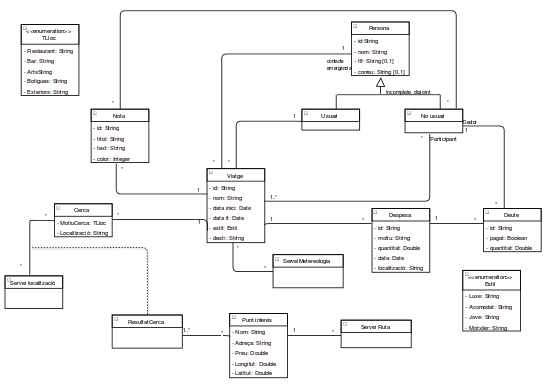
\includegraphics[scale=1]{Figures/UML.png}
\caption{Esquema conceptual.}
\end{figure}


\subsection{Restricions textuals}
\begin{itemize}
\item{}El deutor ha de ser participant del viatge al qual pertany el deute.
\item{}El viatger a qui se li comparteix una nota ha de ser participant del viatge al qual pertany la nota.
\end{itemize}

\clearpage

\subsection{Descripció de les entitats}

\newcolumntype{L}{>{\centering}m{4cm}}
\newcolumntype{M}{m{4cm}}
\newcolumntype{T}{m{7cm}}

\begin{itemize}

\item[]\textbf{Persona}\\
Super classe que s'instància per obtenir una persona de contacte.
\begin{table}[!h]
\centering
\begin{tabular}{|M|T|}
\hline
\textbf{Atribut}  & \textbf{Descripció} \\\hline
Nom &  Nom de la persona\\\hline
Tlf &  Telèfon de la persona\\\hline
Correu &  Correu electrònic de la persona\\\hline
\end{tabular}
\label{}
\caption{Atributs de la classe Persona}
\end{table}

\item[]\textbf{Usuari}\\
Té el rol d'usuari del sistema i és subclasse de Persona.
\begin{table}[!h]
\centering
\begin{tabular}{|M|T|}
\hline
\textbf{Atribut}  & \textbf{Descripció} \\\hline
Nom &  Nom de l'usuari\\\hline
Tlf &  Telèfon de l'usuari\\\hline
Correu &  Correu electrònic de l'usuari\\\hline
\end{tabular}
\label{}
\caption{Atributs de la classe Usuari}
\end{table}

\item[]\textbf{NoUsuari}\\
Té el rol de participant del viatge però sense ser usuari, no interacciona directament amb l'aplicació.

\begin{table}[!h]
\centering
\begin{tabular}{|M|T|}
\hline
\textbf{Atribut}  & \textbf{Descripció} \\\hline
Nom &  Nom del participant\\\hline
Tlf &  Telèfon del participant\\\hline
Correu &  Correu electrònic del participant\\\hline
\end{tabular}
\label{}
\caption{Atributs de la classe NoUsuari}
\end{table}

\item[]\textbf{Viatge}\\
Representa un viatge en concret, és el concepte base de l'aplicació.
\begin{table}[!h]
\centering
\begin{tabular}{|M|T|}
\hline
\textbf{Atribut}  & \textbf{Descripció} \\\hline
Nom &  Nom del viatge\\\hline
Destí &  Destí del viatge\\\hline
Data inici &  Data d'inici del viatge\\\hline
Data fi &  Data final del viatge\\\hline
Estil &  Estil de viatjar seleccionat per l'usuari\\\hline
\end{tabular}
\label{}
\caption{Atributs de la classe Viatge}
\end{table}

\clearpage

\item[]\textbf{Despesa}\\
Representa una despesa de l'usuari durant un viatge.

\begin{table}[!h]
\centering
\begin{tabular}{|M|T|}
\hline
\textbf{Atribut}  & \textbf{Descripció} \\\hline
Motiu &  Motiu de la despesa\\\hline
Quantitat &  Quantiat en euros de la despesa\\\hline
Localització &  Lloc on s'ha generat la despesa\\\hline
Data &  Data de creació de la despesa\\\hline
\end{tabular}
\label{}
\caption{Atributs de la classe Despesa}
\end{table}


\item[]\textbf{Deute}\\
Representa un deute d'un participant del viatge amb l'usuari.

\begin{table}[!h]
\centering
\begin{tabular}{|M|T|}
\hline
\textbf{Atribut}  & \textbf{Descripció} \\\hline
Quantitat & Quantitat del deute en euros.\\\hline
Pagat &  Indica si el deute ja ha estat pagat o no.\\\hline
\end{tabular}
\label{}
\caption{Atributs de la classe Deute}
\end{table}


\item[]\textbf{Nota}\\
Representa una nota escrita per l'usuari.

\begin{table}[!h]
\centering
\begin{tabular}{|M|T|}
\hline
\textbf{Atribut}  & \textbf{Descripció} \\\hline
Títol & Títol de la nota\\\hline
Text &  Text de la nota\\\hline
Color & Color que ha seleccionat l'usuari pel fons de la nota.\\\hline
\end{tabular}
\label{}
\caption{Atributs de la classe Nota}
\end{table}

\item[]\textbf{Cerca}\\
Representa una cerca llençada per l'usuari al sistema.

\begin{table}[!h]
\centering
\begin{tabular}{|M|T|}
\hline
\textbf{Atribut}  & \textbf{Descripció} \\\hline
Motiu & Tipus de cerca, aquest valor pot ser: menjar, begudes, arts, botigues o espais oberts\\\hline
Localització &  Localització des d'on es vol realitzar la cerca\\\hline
\end{tabular}
\label{}
\caption{Atributs de la classe Cerca}
\end{table}


\item[]\textbf{Servei Localització}\\
Representa el servei extern amb qui es comunica el sistema per obtenir resultats en la cerca.


\item[]\textbf{Resultat Cerca}\\
Representa els resultats d'una cerca en concret.

\item[]\textbf{Punt d'interés}\\
Representa un item concret del resultat de la cerca.

\begin{table}[!h]
\centering
\begin{tabular}{|M|T|}
\hline
\textbf{Atribut}  & \textbf{Descripció} \\\hline
Nom & Nom del punt d'interés\\\hline
Adreça &  Adreça del punt d'interés\\\hline
Preu & Nivell de preus del punt d'interés\\\hline
Latitut & Valor de latitut en la localització del punt d'interés\\\hline
Longitut & Valor de longitut en la localització del punt d'interés\\\hline
\end{tabular}
\label{}
\caption{Atributs de la classe Punt d'interés}
\end{table}


\item[]\textbf{Servei Ruta}\\
Representa el servei extern amb qui es comunica el sistema per tal d'obtenir una ruta entre dos punts.

\item[]\textbf{Servei Meteorologia}\\
Representa el servei extern amb qui es comunica el sistema per tal d'obtenir la previsió metereològica.



\end{itemize}

\section{Esquema del comportament}

\newcolumntype{C}{m{10cm}}

\begin{itemize}
\item[]{\textbf{Inici sessió}}

\begin{figure}[!h]
\centering
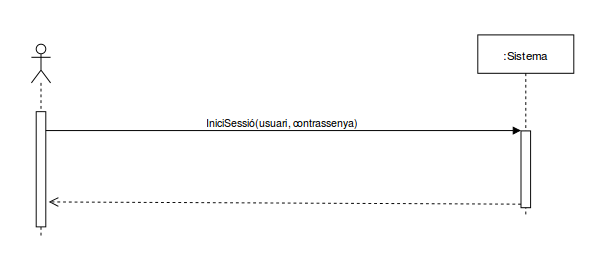
\includegraphics[scale=0.8]{Figures/IniciSessioEC.png}
\end{figure}

\begin{table}[!h]
\centering
\begin{tabular}{l C}
\textbf{Context}  & Sistema::IniciSessió(email:string, contrassenya:string) \\
\textbf{Pre} & email no és buit\\
 & contrassenya no es buida\\
\textbf{Post} &  Si les credencials són correctes l'usuari veu la pantalla de llista dels seus viatges\\
\end{tabular}
\label{}
\end{table}

\clearpage

\item[]{\textbf{Tancar sessió}}

\begin{figure}[!h]
\centering
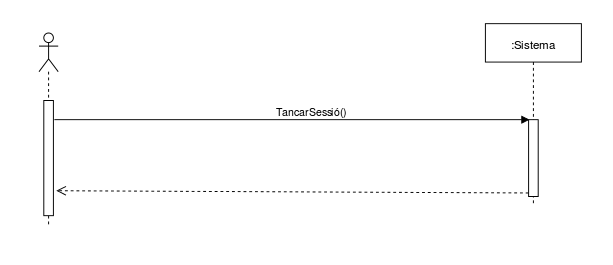
\includegraphics[scale=0.8]{Figures/TancarSessioEC.png}
\end{figure}

\begin{table}[!h]
\centering
\begin{tabular}{l C}
\textbf{Context}  & Sistema::TancarSessio() \\
\textbf{Pre} & L'usuari ha iniciat sessió\\
\textbf{Post} &  L'usuari veu la pantalla d'inici de sessió\\
\end{tabular}
\label{}
\end{table}

\item[]\textbf{Consultar viatge}

\begin{figure}[!h]
\centering
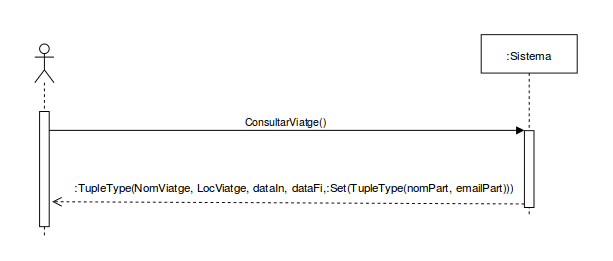
\includegraphics[scale=0.8]{Figures/ConsultarViatgeEC.png}
\end{figure}

\begin{table}[!h]
\centering
\begin{tabular}{l C}
\textbf{Context}  & Sistema::ConsultarViatge():TupleType(NomViatge, LocViatge, dataIn, dataFi,:Set(TupleType(nomPart, emailPart)) \\
\textbf{Pre} & L'usuari ha iniciat sessió\\
\textbf{Post} &  L'usuari veu la pantalla i les dades del viatge\\
\end{tabular}
\label{}
\end{table}

\clearpage

\item[]\textbf{Crear viatge}

\begin{figure}[!h]
\centering
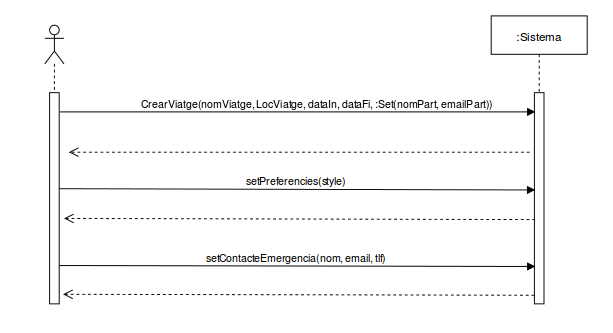
\includegraphics[scale=0.8]{Figures/CrearViatgeEC.png}
\end{figure}

\begin{table}[!h]
\centering
\begin{tabular}{l C}
\textbf{Context}  & Sistema::CrearViatge(nomViatge, LocViatge, dataIn, dataFi, :Set(nomPart, emailPart)) \\
\textbf{Pre} & L'usuari ha iniciat sessió\\
\textbf{Post} &  L'usuari veu la pantalla de seleccionar preferencies de viatge\\
\end{tabular}
\label{}
\end{table}

\begin{table}[!h]
\centering
\begin{tabular}{l C}
\textbf{Context}  & Sistema::SetPreferencies(estil) \\
\textbf{Pre} & L'usuari ha començat la creació d'un viatge\\
\textbf{Post} &  L'usuari veu la pantalla d'introduir les dades del contacte d'emergència\\
\end{tabular}
\label{}
\end{table}

\begin{table}[!h]
\centering
\begin{tabular}{l C}
\textbf{Context}  & Sistema::SetContactesEmergencia(nom, email, tlf) \\
\textbf{Pre} & L'usuari ha seleccionat les preferencies del viatge\\
\textbf{Post} &  S'ha creat el viatge amb totes les dades introduides\\
\end{tabular}
\label{}
\end{table}

\item[]\textbf{Eliminar viatge}

\begin{figure}[!h]
\centering
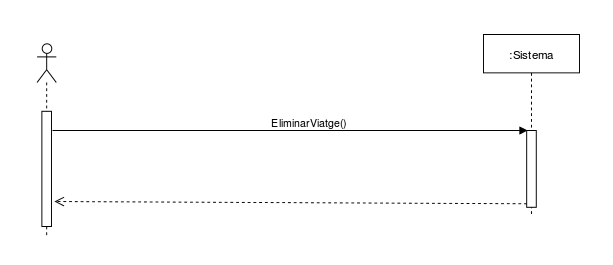
\includegraphics[scale=0.8]{Figures/EliminarViatgeEC.png}
\end{figure}

\clearpage

\begin{table}[!h]
\centering
\begin{tabular}{l C}
\textbf{Context}  & Sistema::EliminarViatge() \\
\textbf{Pre} & L'usuari ha creat un viatge\\
\textbf{Post} &  S'elimina el viatge amb totes les dades associades\\
\end{tabular}
\label{}
\end{table}



\item[]\textbf{Consultar llista de despeses}

\begin{figure}[!h]
\centering
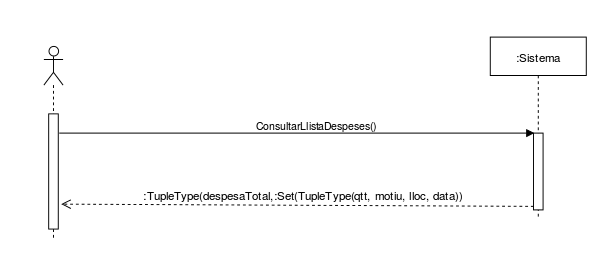
\includegraphics[scale=0.8]{Figures/ConsultarLlistaDespesesEC.png}
\end{figure}

\begin{table}[!h]
\centering
\begin{tabular}{l C}
\textbf{Context}  & Sistema::ConsultarLlistaDespeses():TupleType(despesaTotal,Set(TupleType(qtt, motiu, lloc, data)) \\
\textbf{Pre} & Ha accedit a consultar un viatge\\
\textbf{Post} &  L'usuari veu la pantalla amb la informació de totes les despeses del viatge\\
\end{tabular}
\label{}
\end{table}

\item[]\textbf{Crear despesa}


\begin{figure}[!h]
\centering
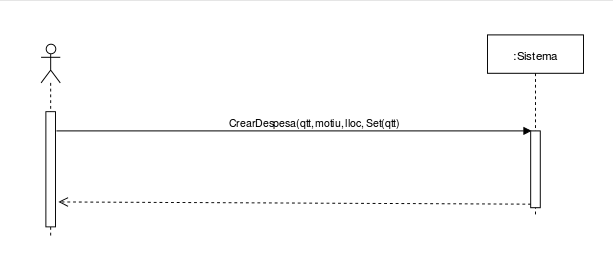
\includegraphics[scale=0.8]{Figures/CrearDespesaEC.png}
\end{figure}

\begin{table}[!h]
\centering
\begin{tabular}{l C}
\textbf{Context}  & Sistema::CrearDespesa(qtt, motiu, lloc, Set(qtt)) \\
\textbf{Pre} & Ha accedit a consultar la llista de despeses\\
\textbf{Post} & Es crea una instància de despesa amb les dades introduides\\
\end{tabular}
\label{}
\end{table}

\clearpage

\item[]\textbf{Consultar despesa}


\begin{figure}[!h]
\centering
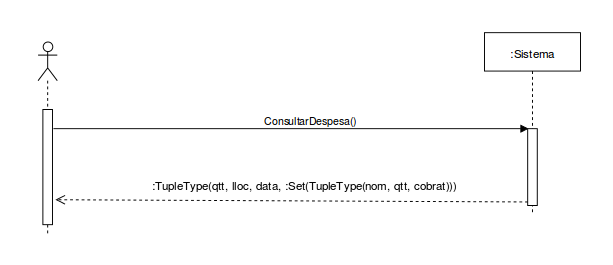
\includegraphics[scale=0.8]{Figures/ConsultarDespesaEC.png}
\end{figure}

\begin{table}[!h]
\centering
\begin{tabular}{l C}
\textbf{Context}  & Sistema::ConsultarDespesa()::TupleType(qtt, lloc, data, Set(TupleType(nom, qtt, cobrat))) \\
\textbf{Pre} & L'usuari ha creat una despesa\\
\textbf{Post} & L'usuari veu la pantalla de consultar despesa amb totes les dades d'aquesta\\
\end{tabular}
\label{}
\end{table}

\item[]\textbf{Cobrar deute}


\begin{figure}[!h]
\centering
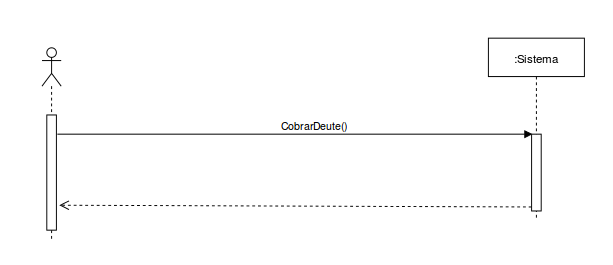
\includegraphics[scale=0.8]{Figures/CobrarDeuteEC.png}
\end{figure}

\begin{table}[!h]
\centering
\begin{tabular}{l C}
\textbf{Context}  & Sistema::CobrarDeute() \\
\textbf{Pre} & L'usuari ha creat una despesa i té un deute pendent de cobrar\\
\textbf{Post} & El sistema enregistra el deute com a cobrat\\
\end{tabular}
\label{}
\end{table}

\clearpage

\item[]\textbf{Eliminar despesa}


\begin{figure}[!h]
\centering
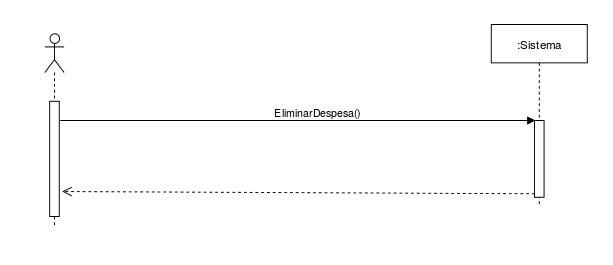
\includegraphics[scale=0.8]{Figures/EliminarDespesaEC.png}
\end{figure}

\begin{table}[!h]
\centering
\begin{tabular}{l C}
\textbf{Context}  & Sistema::EliminarDespesa() \\
\textbf{Pre} & L'usuari ha creat una despesa\\
\textbf{Post} & El sistema elimina la despesa i tots els deutes associats\\
\end{tabular}
\label{}
\end{table}

\item[]\textbf{Modificar despesa}


\begin{figure}[!h]
\centering
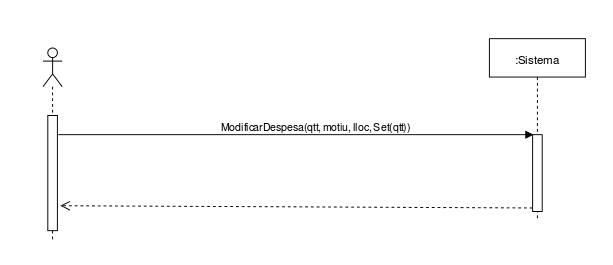
\includegraphics[scale=0.8]{Figures/ModificarDespesaEC.png}
\end{figure}

\begin{table}[!h]
\centering
\begin{tabular}{l C}
\textbf{Context}  & Sistema::ModificarDespesa(qtt, motiu, lloc, Set(qtt)) \\
\textbf{Pre} & L'usuari ha creat una despesa\\
\textbf{Post} & El sistema modifica la despesa amb els nous paràmetres introduits\\
\end{tabular}
\label{}
\end{table}

\clearpage

\item[]\textbf{Cerca}

\begin{figure}[!h]
\centering
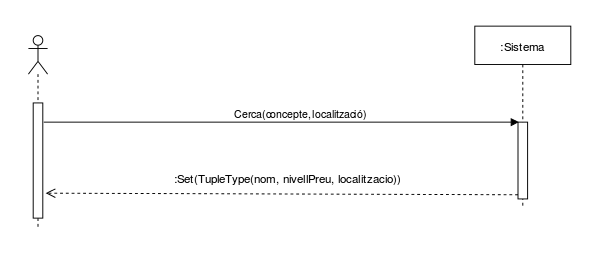
\includegraphics[scale=0.8]{Figures/CercaEC.png}
\end{figure}

\begin{table}[!h]
\centering
\begin{tabular}{l C}
\textbf{Context}  & Sistema::Cerca(concepte, localització):Set(TupleType(nom, nivellPreu, localitzacio)) \\
\textbf{Pre} & L'usuari ha accedit a consultar un viatge\\
\textbf{Post} & L'usuari veu la llista de resultats de la cerca\\
\end{tabular}
\label{}
\end{table}

\item[]\textbf{Consultar ruta}

\begin{figure}[!h]
\centering
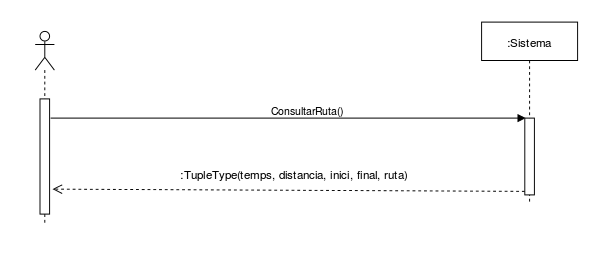
\includegraphics[scale=0.8]{Figures/ConsultarRutaEC.png}
\end{figure}

\begin{table}[!h]
\centering
\begin{tabular}{l C}
\textbf{Context}  & Sistema::ConsultarRuta():TupleType(temps, distancia, inici, final, ruta) \\
\textbf{Pre} & L'usuari ha realitzat una cerca\\
\textbf{Post} & L'usuari veu la pantalla de consultar ruta amb tota la informació de la ruta\\
\end{tabular}
\label{}
\end{table}

\clearpage

\item[]\textbf{Consultar Meteorologia}

\begin{figure}[!h]
\centering
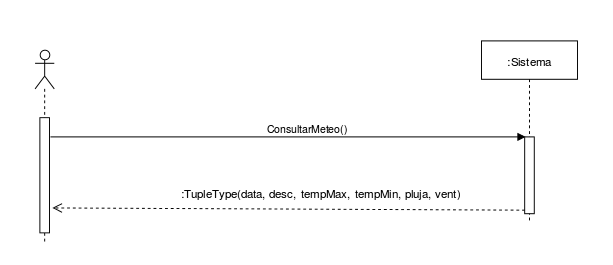
\includegraphics[scale=0.8]{Figures/ConsultarMeteoEC.png}
\end{figure}

\begin{table}[!h]
\centering
\begin{tabular}{l C}
\textbf{Context}  & Sistema::ConsultarMeteo():TupleType(data, desc, tempMax, tempMin, pluja, vent)\\
\textbf{Pre} & L'usuari ha accedit a consultar un viatge\\
\textbf{Post} & L'usuari veu la pantalla de consultar metereologia amb tota la informació de la previsió metereològica\\
\end{tabular}
\label{}
\end{table}

\item[]\textbf{Consultar ruta a l'hospital}

\begin{figure}[!h]
\centering
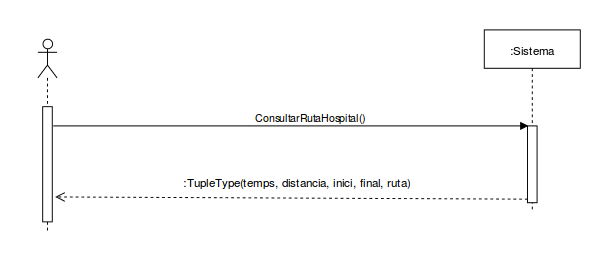
\includegraphics[scale=0.8]{Figures/ConsultarRutaHospitalEC.png}
\end{figure}

\begin{table}[!h]
\centering
\begin{tabular}{l C}
\textbf{Context}  & Sistema::ConsultarRutaHospital():TupleType(temps, distancia, inici, final, ruta)\\
\textbf{Pre} & L'usuari ha accedit a la funcionalitat de gestionar emergències\\
\textbf{Post} & L'usuari veu a la pantalla la ruta fins l'hospital més proper i tota la informació adicional\\
\end{tabular}
\label{}
\end{table}

\clearpage

\item[]\textbf{Trucar telèfon d'emergències}

\begin{figure}[!h]
\centering
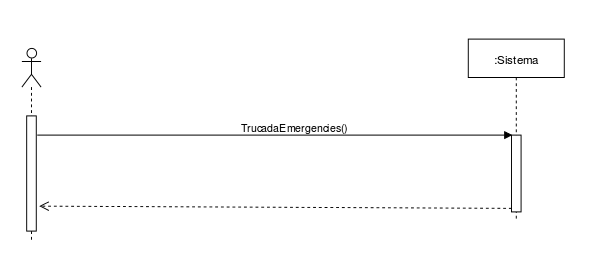
\includegraphics[scale=0.8]{Figures/TrucadaEmergenciesEC.png}
\end{figure}

\begin{table}[!h]
\centering
\begin{tabular}{l C}
\textbf{Context}  & Sistema::TrucadaEmergencies()\\
\textbf{Pre} & L'usuari ha accedit a la funcionalitat de gestionar emergències\\
\textbf{Post} & El sistema realitza una trucada al telèfon d'emergències del país on es troba l'usuari\\
\end{tabular}
\label{}
\end{table}

\item[]\textbf{Trucar telèfon de contacte}

\begin{figure}[!h]
\centering
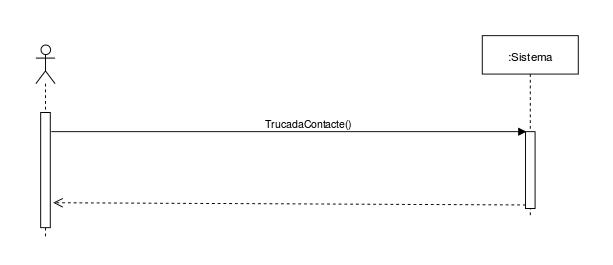
\includegraphics[scale=0.8]{Figures/TrucadaContacteEC.png}
\end{figure}

\begin{table}[!h]
\centering
\begin{tabular}{l C}
\textbf{Context}  & Sistema::TrucadaContacte()\\
\textbf{Pre} & L'usuari ha accedit a la funcionalitat de gestionar emergències\\
\textbf{Post} & El sistema realitza una trucada al telèfon de contacte introduit per l'usuari\\
\end{tabular}
\label{}
\end{table}

\clearpage

\item[]\textbf{Consultar llista de notes}

\begin{figure}[!h]
\centering
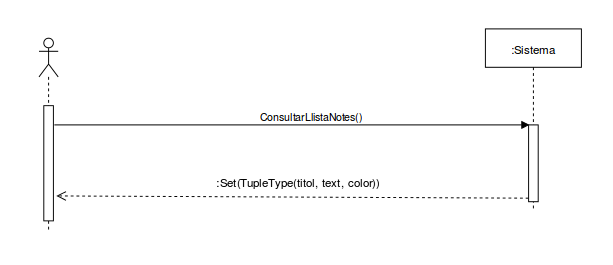
\includegraphics[scale=0.8]{Figures/ConsultarLlistaNotesEC.png}
\end{figure}

\begin{table}[!h]
\centering
\begin{tabular}{l C}
\textbf{Context}  & Sistema::ConsultarLlistaNotes():Set(TupleType(titol, text, color))\\
\textbf{Pre} & L'usuari ha accedit a consultar un viatge\\
\textbf{Post} & L'usuari veu la pantalla amb totes les notes del viatge\\
\end{tabular}
\label{}
\end{table}

\item[]\textbf{Consultar nota}

\begin{figure}[!h]
\centering
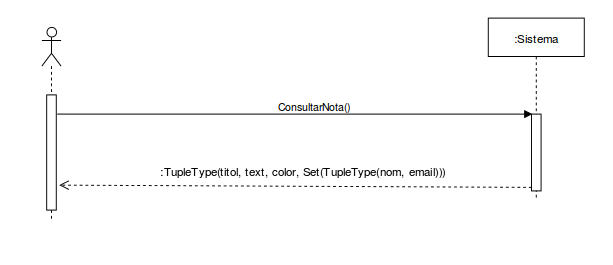
\includegraphics[scale=0.8]{Figures/ConsultarNotaEC.png}
\end{figure}

\begin{table}[!h]
\centering
\begin{tabular}{l C}
\textbf{Context}  & Sistema::ConsultarNota():TupleType(titol, text, color, Set(TupleType(nom, email)))\\
\textbf{Pre} & L'usuari ha consultar la llista de notes\\
\textbf{Post} & L'usuari veu la pantalla de consultar nota amb tota la informació d'aquesta\\
\end{tabular}
\label{}
\end{table}

\clearpage

\item[]\textbf{Crear nota}

\begin{figure}[!h]
\centering
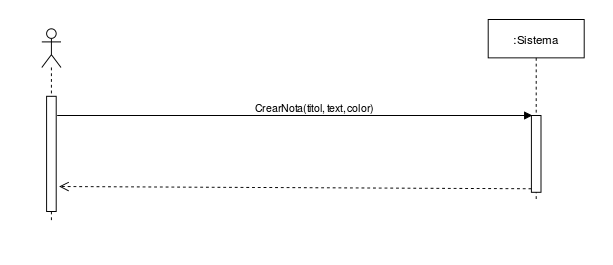
\includegraphics[scale=0.8]{Figures/CrearNotaEC.png}
\end{figure}

\begin{table}[!h]
\centering
\begin{tabular}{l C}
\textbf{Context}  & Sistema::CrearNota(titol, text, color)\\
\textbf{Pre} & L'usuari ha accedit a consultar la llista de notes\\
\textbf{Post} & El sistema crea una instància de nota amb les dades introduides i l'usuari veu la pantalla de consultar nota\\
\end{tabular}
\label{}
\end{table}

\item[]\textbf{Eliminar nota}

\begin{figure}[!h]
\centering
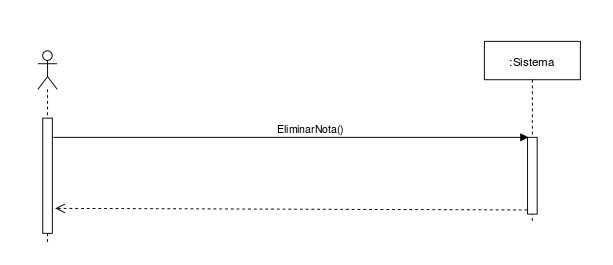
\includegraphics[scale=0.8]{Figures/EliminarNotaEC.png}
\end{figure}

\begin{table}[!h]
\centering
\begin{tabular}{l C}
\textbf{Context}  & Sistema::EliminarNota()\\
\textbf{Pre} & L'usuari ha accedit a consultar una nota\\
\textbf{Post} & El sistema elimina la nota\\
\end{tabular}
\label{}
\end{table}

\end{itemize}
